\documentclass{article}

% if you need to pass options to natbib, use, e.g.:
% \PassOptionsToPackage{numbers, compress}{natbib}
% before loading nips_2017
%
% to avoid loading the natbib package, add option nonatbib:
% \usepackage[nonatbib]{nips_2017}

\usepackage{nips_2017}

% to compile a camera-ready version, add the [final] option, e.g.:
% \usepackage[final]{nips_2017}

\usepackage[utf8]{inputenc} % allow utf-8 input
\usepackage[T1]{fontenc}    % use 8-bit T1 fonts
%\usepackage{hyperref}       % hyperlinks
\usepackage[hidelinks]{hyperref}
\usepackage{url}            % simple URL typesetting
\usepackage{booktabs}       % professional-quality tables
\usepackage{amsfonts}       % blackboard math symbols
\usepackage{nicefrac}       % compact symbols for 1/2, etc.
\usepackage{microtype}      % microtypography
\usepackage{amsmath}
\usepackage{subcaption}
\usepackage{graphicx}
%\usepackage{subfigure}

\newenvironment{mycell}[1]
{
	\begin{minipage}{#1}
		\begin{center}
			\vspace*{0.15cm}
		}
		{
			\vspace*{0.1cm}
		\end{center}
	\end{minipage}
}

\title{Generalised Training of Spiking Neural Networks}

% The \author macro works with any number of authors. There are two
% commands used to separate the names and addresses of multiple
% authors: \And and \AND.
%
% Using \And between authors leaves it to LaTeX to determine where to
% break the lines. Using \AND forces a line break at that point. So,
% if LaTeX puts 3 of 4 authors names on the first line, and the last
% on the second line, try using \AND instead of \And before the third
% author name.

\author{
	David S.~Hippocampus\thanks{Use footnote for providing further
		information about author (webpage, alternative
		address)---\emph{not} for acknowledging funding agencies.} \\
	Department of Computer Science\\
	Cranberry-Lemon University\\
	Pittsburgh, PA 15213 \\
	\texttt{hippo@cs.cranberry-lemon.edu} \\
	%% examples of more authors
	%% \And
	%% Coauthor \\
	%% Affiliation \\
	%% Address \\
	%% \texttt{email} \\
	%% \AND
	%% Coauthor \\
	%% Affiliation \\
	%% Address \\
	%% \texttt{email} \\
	%% \And
	%% Coauthor \\
	%% Affiliation \\
	%% Address \\
	%% \texttt{email} \\
	%% \And
	%% Coauthor \\
	%% Affiliation \\
	%% Address \\
	%% \texttt{email} \\
}

\begin{document}
	% \nipsfinalcopy is no longer used
	
	\maketitle
	
	\begin{abstract}
		%	To train time-based, biologically-plausible spiking neural networks~(SNNs) on conventional artificial neural networks~(ANNs), 
		Spiking neural networks~(SNNs) can be trained by first training an equivalent ANN and then transferring the trained weights to the SNN, but there are two significant problems to be solved.
		First, an accurate activation function is needed to model the neural dynamics of spiking neurons, and our previously proposed activation function, Noisy Softplus, has shown to be a good match to the response activity of Leaky Integrate-and-Fire~(LIF) neurons.
		The second problem is mapping the abstract numerical values of the ANN to concrete physical units in the SNN, such as current and firing rate.
		In this paper, we introduce the parametric activation function~[PAF; $f_{P}(x) = p \times f(x)$], to tackle the second problem.
%		With these problems solved, SNNs can be trained exactly the same way as ANNs, and the trained weights can be used directly in the spiking version of the same network without any conversion.
%		More importantly, the PAF can be generalised to activation functions other than Noisy Softplus, such as the Rectified Linear Unit~(ReLU).%, and the parameters are independent to activation functions.
		With these problems solved, SNN training can be simplified as: (1) estimate parameter $p$ for PAF according to biological configurations of LIF neurons, and (2) use PAF instead of conventional activation functions to train an equivalent ANN.
		The trained weights can be transferred directly into the spiking version of the same network without further conversion.
		In addition, we propose a fine tuning method as an option which helps the trained network to closer match the SNN.
		Based on this generalised training method, we achieve the best SNN accuracy on the MNIST task using LIF neurons, 98.85\%, on a 6-layer spiking convolutional neural network~(ConvNet).
		
		
		
		%  We extended the work of proposed activation function, Noisy Softplus, to fit into training of layered up deep spiking neural networks~(SNNs).
		%  Thus, a time-dependant, biologically-plausible spiking neuron can be modelled as a traditional rate-based neuron in artificial neural networks~(ANNs).
		%  Such an ANN can be trained simply by the traditional algorithm, for example Back Propagation~(BP), and the trained weights can be directly used in the spiking version of the same network without any conversion.
		%  Furthermore, the training method has been generalised to other activation units, for instance Rectified Linear Units (ReLU), to train deep SNNs off-line.
		%  This research is crucial to provide a generalised SNN training method, to improve the learning ability of SNNs with biological characteristics, and to close the gap towards equivalent performance as ANNs.
		
	\end{abstract}
	
	\section{Introduction}
	Advances in computing power and deep learning have benefited computers with a rapidly growing performance in cognitive tasks, such as recognising objects~\cite{deng2009imagenet} and playing GO~\cite{silver2016mastering}. 
	These tasks were once dominated by human intelligence and solved by biological neurons in the brain.
	However, humans and many other animals still win against computers in practical tasks and outperform in the terms of size and energy by several orders of magnitude.
	For instance, AlphaGO~\cite{silver2016mastering} consumed 1~MW of power on its 1920 CPUs and 280 GPUs when playing the game with one of the best human players whose brain merely consumed about 20~W.
	Although we are still far from understanding the brain thoroughly, it is believed that the performance gap between computation in the biological nervous system and in a computer lies in the fundamental computing units and how these compute.
	Computers employ Boolean logic and deterministic digital operations based usually on synchronous clocks while nervous systems employ parallel-distributed, event-driven, stochastically unreliable components~\cite{indiveri2009artificial}, neurons.
	The impressive disparities in cognitive capabilities and energy consumption drives the research into biologically-plausible spiking neurons and brain inspired computers, known as neuromorphic engineering~\cite{furber2016bio}.
	
	A regular artificial neuron (Figure~\ref{Fig:compare_as}(a)) comprises a weighted summation of input data, $\sum x_i w_i$, and an activation function, $f$, applied on the sum.
	Usually, a bias is included in the weighted summation which can be seen as an extra input $x_b = 1$ with its weight set to $b$.
	However, in this paper we exclude biases for both artificial and spiking neurons to simplify neural models and to reduce the number of parameters.
%	Meanwhile the inputs of a spiking neuron (Figure~\ref{Fig:compare_as}(b)) are pre-synaptic spike trains, which create post-synaptic potentials~(PSPs) and trigger spikes as outcomes when the neuron's membrane potential reaches some threshold.
	Meanwhile the inputs of a spiking neuron (Figure~\ref{Fig:compare_as}(b)) are spike trains, which generates current influx through neural synapses (connections).
	A single spike creates a current pulse with an amplitude of $w$, which is defined as the synaptic efficacy, and the current then decays exponentially with a decaying rate determined by the synaptic time constant, $\tau_{syn}$.
	The current pulses then consequently produce post-synaptic potentials~(PSPs) on the neuron driving its membrane potential change over time, and trigger spikes as outcomes when the neuron's membrane potential reaches some threshold.
	The dynamics of the current influxes, PSPs, membrane potentials, and spike trains are all time dependent, while neurons of ANNs only cope with abstract numerical values representing spiking rate, without timing information.
	These fundamental differences in input/output representation and neural computation raise the research problem of how to operate and train biologically-plausible SNNs to make them as competent as ANNs in cognitive tasks.
	
	\begin{figure}[tb!]
		\centering
		\begin{subfigure}[t]{0.32\textwidth}
			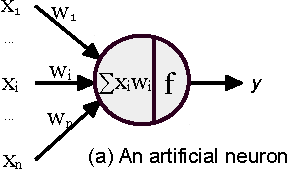
\includegraphics[width=\textwidth]{pics_iconip/neuron_ann.pdf}
			%			\caption{Current sampled at $dt$=1~ms.}
		\end{subfigure}~
		\begin{subfigure}[t]{0.65\textwidth}
			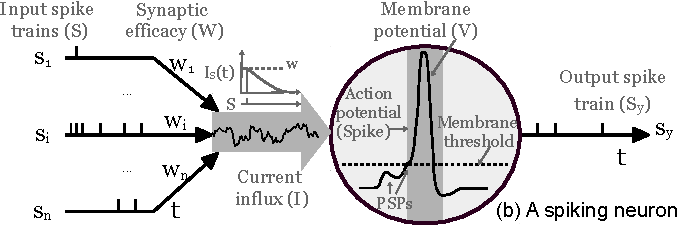
\includegraphics[width=\textwidth]{pics_iconip/neuron_snn.pdf}
			%			\caption{Current sampled at $dt$=10~ms.}
		\end{subfigure}
		\caption{Comparison of the processing mechanisms of an artificial and a spiking neuron. (a) An artificial neuron takes numerical values of vector \textbf{x} as input, performs a weighted summation followed by an activation function $f$. (b) Spike trains flow into a spiking neuron as current influx, trigger linearly summed PSPs through synapses with different synaptic efficacy \textbf{w}, and the post-synaptic neuron generates output spikes when the membrane potential reaches some threshold.}
		\label{Fig:compare_as}
	\end{figure}
	
	An intuitive idea is to train SNNs on an equivalent ANN and then transfer the trained weights to the SNN.
	Jug et al.~\cite{Jug_etal_2012} first proposed the use of the Siegert formula~\cite{siegert1951first} as the activation function in training Deep Belief Networks, which maps incoming currents driven by Poisson spike trains to the response firing rate of an LIF neuron.
	The variables of the activation function are in physical units, thus the trained weights can be transferred directly into SNNs.
	%Jug et al\cite{Jug_etal_2012} first proposed the use of the Siegert function to replace the sigmoid activation function in training Restricted Boltzmann Machines (RBMs).
	%The Siegert units map incoming currents driven by Poisson spike trains to the response firing rate of an LIF neuron.
	%The ratio of the spiking rate to its maximum is equivalent to the output of a sigmoid neuron.
	%A spiking Deep Belief Network (DBN)~\cite{Stromatias2015scalable} of four layers of RBMs was implemented on neuromorphic hardware, SpiNNaker~\cite{furber2014spinnaker}, to recognise hand written digits in real time.
	However, the Siegert formula is inaccurate as it models the current noise as white~\cite{liu2016noisy}, $\tau_{syn} \to 0$, but it is not feasible in practice.
%	taking no notice of the coloured noise generated by the synaptic time constant $\tau_{syn}$ of spike arrivals, since the current noise is only a white noise when $\tau_{syn} \to 0$~.
	Moreover, the high complexity of the Siegert function and the computation of its derivative to obtain the error gradient cause much longer training time, thus consuming more energy, when compared to regular ANN activation functions, such as Sigmoid.
	%Additionally, neurons have to fire at high frequency (higher than half of the maximum firing rate) to represent the activation of a sigmoid unit; thus the network activity results in high power dissipation.
	%Hence researchers turned to abstract activation functions to model the response activity of spiking neurons to simplify the computation. %and at the same time improve the model accuracy of the activation function.
%	A similar activation function of Soft LIF~\cite{hunsberger2015spiking} was introduced to simplify the computation complexity.
	A softened version of the response function of LIF neurons is proposed~\cite{hunsberger2015spiking} and is less computationally expensive than the Siegert function.
	However, the model ignored the dynamic noise change introduced by input spikes, assuming static noise level of the current influx.
	Therefore the training required additional noise on the response firing rate and on the training data, thus included hyper-parameters in the model.
%	What's more, the activation function compromised the modelling accuracy for computational simplicity.
	
	
	Therefore, the first problem is the accurate modelling of the neural response activity of LIF neurons using abstract activation functions, in the hope of (1) increasing the performance of SNN training and (2) reducing the computation complexity.
	We call activation functions `abstract' referring to the ones without physical units which are used in the ANNs, and select them for LIF modelling due to their simplicity and generalised use for training of ANNs.
	Noisy Softplus~\cite{liu2016noisy}, proved to be a close match to the response activity of LIF neurons by including current noise as the second factor in the activation function and taking account of coloured noise driven by $\tau_{syn}$.
	
	
	Then the second problem is to map the abstract activation functions to physical units: current in \textit{nA} and firing rates in \textit{Hz}. 
	%Better learning performance has been reported using ReLU, so modelling ReLU-like activation function for spiking neurons is needed.  
	%Based on the fact that cortical neurons seldom saturate their firing rate as sigmoid neurons,ReLU~\cite{glorot2011deep} were proposed to replace sigmoid neurons and surpassed the performance of other popular activation units.
	%trained with noisy input, the 4-layered spiking autoencoder reached 98.37\% accuracy on MNIST. 
	Instead of solving this problem, an alternative way of converting ANN-trained weights for use in SNNs~\cite{cao2015spiking,diehl2015fast} was successfully applied 
	on less biologically-realistic and simplified integrate-and-fire (IF) neurons.
	Normalising the ReLU-trained weights for use on simplified IF neurons was relatively straightforward, so this method sets the state-of-the-art performance.
	However, this paper aims to address the second problem of mapping activation functions to the response firing activity of biologically-plausible LIF neurons, thus to complete a formalised SNN training mechanism and to generalise the method to commonly-used simple activation functions, such as ReLU.
	
	
	%Recent developments on ANN-trained SNN models has focused on using ReLU units and converting trained weights to fit in SNNs.
	%Better performance~\cite{cao2015spiking,diehl2015fast} than Siegert-trained RBM has been demonstrated in spiking ConvNets.
	%But this training method employed less biologically-realistic and simplified integrate-and-fire (IF) neurons.
	%The training used only ReLUs and zero bias to avoid negative outputs, and applied a deep learning technique, dropout\cite{srivastava2014dropout} , to increase the classification accuracy.
	
	%This work was extended to a Recursive Neural Network (RNN)~\cite{diehl2016conversion} and run on the TrueNorth\cite{merolla2014million} neuromorphic hardware platform.
	
	%Except for the popular, simplified version of ReLU, $max(0,\sum w x)$, the other implementation of $\log(1+e^x)$, ``Softplus'', is more biologically realistic.
	%Recent work~\cite{hunsberger2015spiking} proposed the Soft LIF response function for training SNNs, which is equivalent to Softplus activation of ANNs.
	%Furthermore, neuroscientific study has showed that the spike train of individual neurons is far from being periodic, which thus brings noisy to the input signal of spiking neurons~\cite{Gerstner:2002}.
	
	
	%Therefore, in the previous work of Qian Liu et al.~\cite{liu2016noisy}, the difference between analytical estimation and practical simulations of spiking neurons were compared, and a new activation function named Noisy Softplus was proposed to match the response function of LIF neurons. In order to close the gap between the performance of SNNs and ANNs, and to further improve the performance of SNNs, we extended Noisy Softplus with a scale factor and proposed a complete layered up SNN training method by using artificial neurons of combined activation.
	
	This paper will start with a brief review on modelling the LIF response function with Noisy Softplus in Section~\ref{sec:back}, and introduce the PAF in Section~\ref{sec:meth} to address the second problem mentioned above and complete the generalised SNN training method.
	In Section~\ref{sec:result} we will demonstrate the training of a spiking ConvNet, and compare the proposed method to existing training algorithms.
	
	\section{Background}
	\label{sec:back}
	\begin{figure}[thb!]
		\centering
		\begin{subfigure}[t]{0.4\textwidth}
			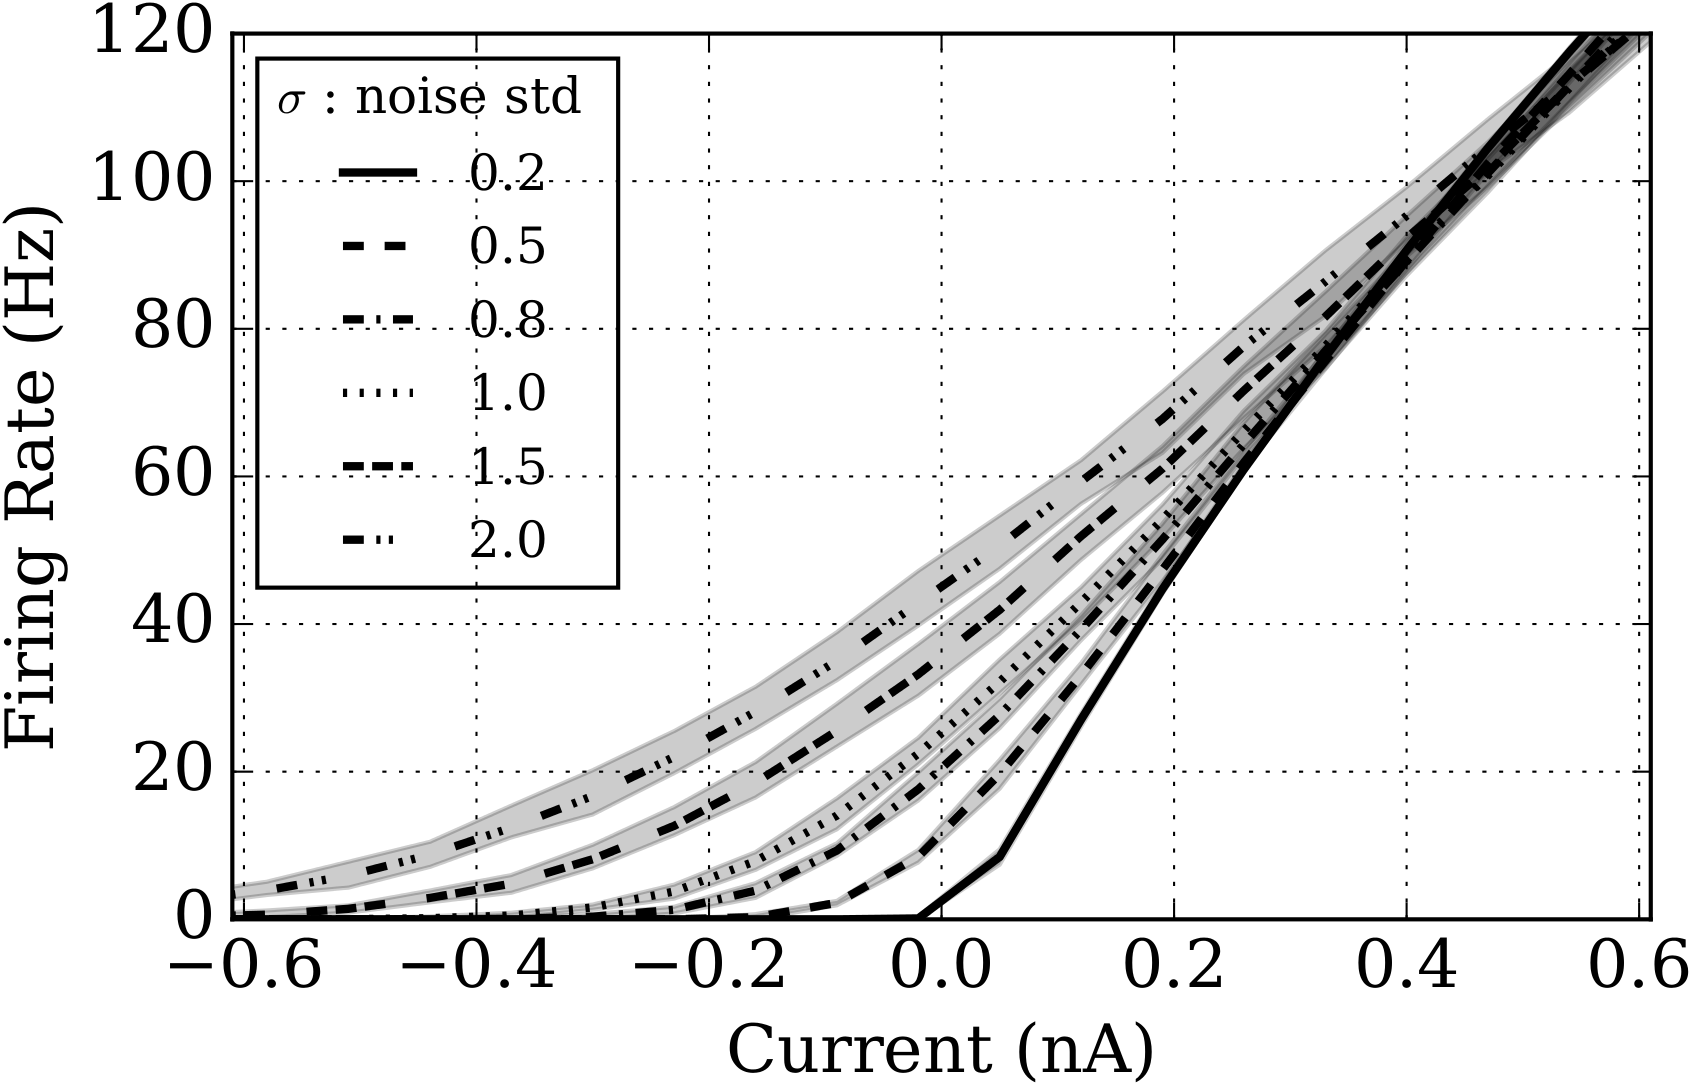
\includegraphics[width=\textwidth]{pics_iconip/siegert.png}
			\caption{Response firing rate of an LIF neuron}
		\end{subfigure}~~~~~~
		\begin{subfigure}[t]{0.4\textwidth}
			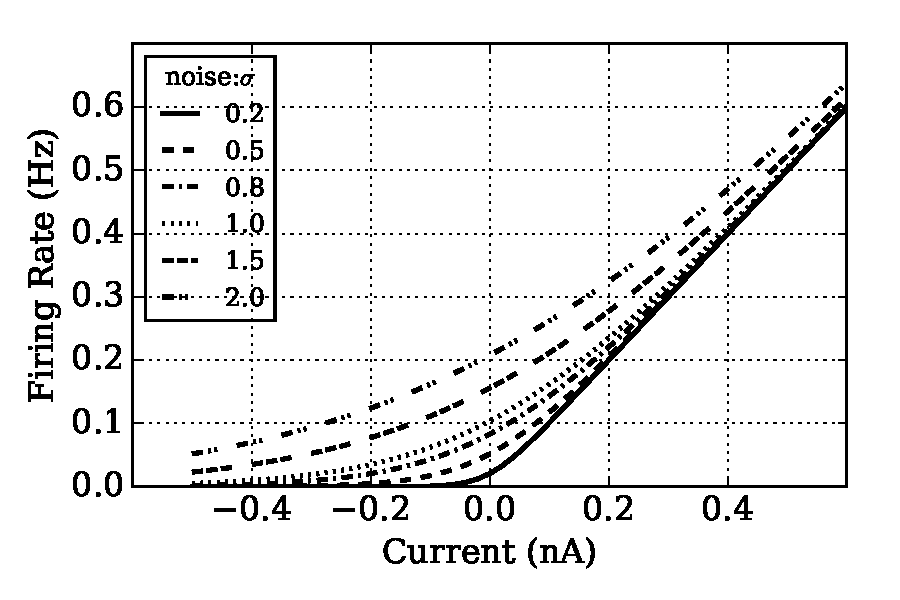
\includegraphics[width=\textwidth]{pics_iconip/4.pdf}
			\caption{Noisy Softplus}
		\end{subfigure}
		\caption{
			%		Noisy Softplus fits to the response function of the LIF neuron.
			Noisy Softplus models the LIF response function.
			(a) Firing rates measured by simulations on an LIF neuron driven by different input currents and discrete noise levels.
			Bold lines show the average and the grey colour fills the range between the minimum and the maximum.
			(b) Noisy Softplus activates the input $x$ according to different noise levels where $k=0.16$.}
		\label{fig:ns}
	\end{figure}
	To model the response function of LIF neurons (see Figure~\ref{fig:ns}(a)) whose output firing rates are determined by the mean and variance of the noisy input currents, we proposed the Noisy Softplus:
	\begin{equation}
	y = f_{ns}(x, \sigma) = k \sigma \log [1 + \exp(\frac{x}{k \sigma})]~,
	\label{equ:nsp}
	\end{equation}
	where $x$ and $\sigma$ refer to the mean and standard deviation of the input current, $y$ indicates the intensity of the output firing rate, and $k$, determined by the biological configurations on the LIF neurons~\cite{liu2016noisy}~(listed in Table~\ref{tbl:pynnConfig}), controls the shape of the curves.
	Note that the novel activation function we proposed contains two parameters, the mean current and its noise, which can be estimated by:
	\begin{equation}
	x = \tau_{syn}\sum_i w_i\lambda_{i}~, ~\sigma^2=\frac{1}{2}\tau_{syn}\sum_i w_i^2\lambda_{i}~,
	\label{equ:distr}
	\end{equation}
	where $\lambda_i$ indicates the firing rate of an input spike train.
	%; both are naturally obtained in spiking neurons.
	% With doubled information, more powerful training methods and network models are expected. 
	Figure~\ref{fig:ns}(b) shows the activation function in curve sets corresponding to different discrete noise levels which mimic the responding activities of LIF neurons.
	The derivative of the Noisy Softplus is the logistic function scaled by $k\sigma$:
	\begin{equation}
	\frac{\partial f_{ns}(x,\sigma)}{\partial x} = \frac{1}{1+exp(-\frac{x}{k\sigma})}~~,
	\label{equ:logist}
	\end{equation}	
	which could be applied easily to back propagation in any ANN training.
	
	\begin{table}[thb]
		\centering
		\caption{\label{tbl:pynnConfig}Default parameter settings for the current-based LIF neurons used through this paper, for PyNN~\cite{davison2008pynn} simulations.}
		\bgroup
		\def\arraystretch{1.4}
		\begin{tabular}{c c c c c c c}
			%\hline
			cm & tau\_m & tau\_refrac & v\_reset & v\_rest& v\_thresh & i\_offset \\
			\hline
			0.25 nF & 20.0 ms & 1.0 ms & -65.0 mV & -65.0 mV & -50.0 mV &  0.1 nA 
		\end{tabular}
		\egroup
	\end{table}
	
	
	\section{Methods}	
	\label{sec:meth}
	
	\subsection{Mapping Noisy Softplus to Concrete Physical Units}
	\label{sec:af_model}
	The inputs of the Noisy Softplus, $x$ and $\sigma$, are obtained from physical variables as stated in Equation~\ref{equ:distr}, thus they are already in physical units (\textit{nA}).
	Therefore, linearly scaling up the activation function by a factor~$S$~(\textit{Hz}/\textit{nA}) can approximate the output firing rate $\lambda_{out}$ of an LIF neuron in \textit{Hz}:
	\begin{equation}
	\lambda_{out} \simeq f_{ns}(x, \sigma) \times S = k \sigma \log [1 + \exp(\frac{x}{k \sigma})] \times S~.
	\label{equ:fit}
	\end{equation}	
	
	
	Suitable calibrations of $k$ and $S$ in Equation~\ref{equ:fit} enables Noisy Softplus to closely match the practical response firing rates of LIF neurons given various biological parameters.
	The parameter pair of $(k, S)$ is curve-fitted with the triple data points of $(\lambda_{out}, x, \sigma)$ and the calibration currently is conducted by linear least squares regression.
	The output firing rate $\lambda_{out}$ is measured from SNN simulations where an LIF neuron is driven by synaptic input current of Poisson spike trains.
	Figure~\ref{Fig:nsptau1} shows two calibration results in which 
	the parameters were fitted to $(k, S)=(0.19,208.76)$ when the synaptic constant is set to $\tau_{syn}=1$~ms and fitted to $(k, S)=(0.35,201.06)$ when $\tau_{syn}=10$~ms.
	%numerical analysis is considered however for future work to express the factors with biological parameters of an LIF neuron.
	
	\begin{figure}
		\centering
		\begin{subfigure}[t]{0.48\textwidth}
			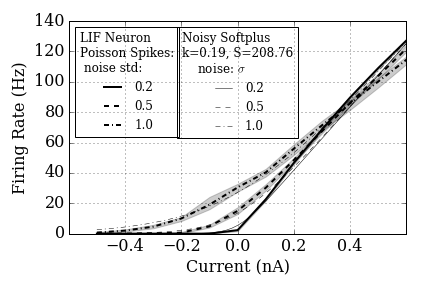
\includegraphics[width=\textwidth]{pics_iconip/4-1.png}
			\caption{$\tau_{syn}$=1~ms}
		\end{subfigure}
		\begin{subfigure}[t]{0.48\textwidth}
			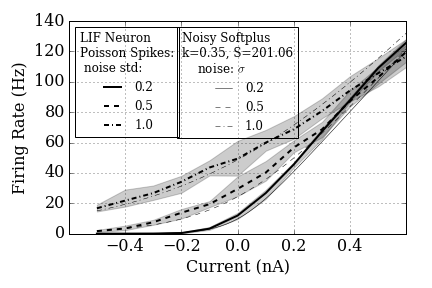
\includegraphics[width=\textwidth]{pics_iconip/4-10.png}
			\caption{$\tau_{syn}$=10~ms}
		\end{subfigure}
		\caption{Noisy Softplus fits to the response firing rates of LIF neurons in concrete physical units.
		Recorded response firing rate of an LIF neuron driven by synaptic current with two synaptic time constants: (a) $\tau_{syn}$=1~ms and (b) $\tau_{syn}$=10~ms. Averaged firing rates of simulation trails are shown in bold lines, and the grey colour fills the range between the minimum to maximum of the firing rates. The thin lines are the scaled Noisy Softplus.}
		\label{Fig:nsptau1}
	\end{figure}
	
	\subsection{Parametric Activation Functions~(PAFs)}
	\begin{figure}[tbh!]
		\centering
		\begin{subfigure}[t]{0.49\textwidth}
			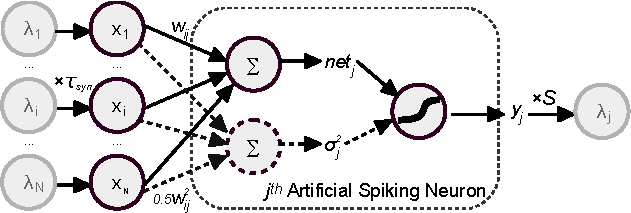
\includegraphics[width=\textwidth]{pics_iconip/neuron_o.pdf}
			\caption{Noisy Softplus}
		\end{subfigure}~~~
		\begin{subfigure}[t]{0.42\textwidth}
			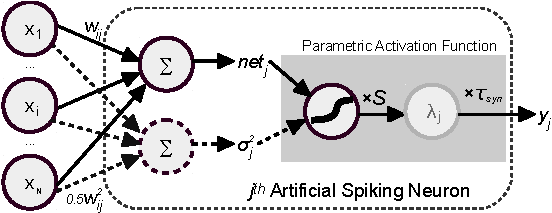
\includegraphics[width=\textwidth]{pics_iconip/neuron_PAF.pdf}
			\caption{Parametric Noisy Softplus}
		\end{subfigure}
		\caption{The PAF links the firing activity of a spiking neuron to the numerical value of ANNs.}
		\label{Fig:tneuron}
	\end{figure}
	
	
	Neurons in ANNs take inputs from their previous layer, and feed the weighted sum of their input, $net_j = \sum_i w_{ij}x_i$, to the activation function.
	The transformed signal then forms the output of an artificial neuron, which can be denoted as $y_j=f(net_j)$, see Figure~\ref{Fig:compare_as}(a).
	However, a spiking neuron modelled by Noisy Softplus takes the firing rate as its input/output, thus Equation~\ref{equ:distr} can be written as:
	\begin{equation}
	net_j = \sum_i w_{ij}(\lambda_{i}\tau_{syn})~,
	~\sigma^2_j= \sum_i (\frac{1}{2} w_{ij}^2)(\lambda_{i}\tau_{syn})~, 
	% \textrm{~~and~~} x_i = \lambda_{i}\tau_{syn}~.
	\label{equ:mi_input}
	\end{equation}
	and input $ x_i $ of an artificial neuron can be seen as $x_i=\lambda_{i}\tau_{syn}$, see Figure~\ref{Fig:tneuron}(a).
	
	If instead of multiplying every input by $\tau_{syn}$ [left of Fig.~\ref{Fig:tneuron}(a)] we do it in every output after $\lambda_j$, [right of Fig.~\ref{Fig:tneuron}(b)] we obtain the same neuron model and structure as a typical neuron in ANNs, See Figure~\ref{Fig:compare_as}(a), that neurons take $x$ as input and output $y$.
%	The PAF version of the activation function (Eq.~\ref{equ:PAF}) will be linearly-scaled by the conversion parameter $S$ and the synaptic time constant $\tau_{syn}$:
	The only difference lies in the activation function where the artificial spiking neuron takes PAF, which is a simple linearly-scaled activation function with a parameter $p$, which is determined by the product of the scaling parameter $S$ and the synaptic time constant $\tau_{syn}$:
	\begin{equation}
	y = p \times f(x) = S \times \tau_{syn} \times f(x)~,
	\label{equ:PAF}
	\end{equation}
	and its derivative function, which is used for back propagation, is:
	\begin{equation}
	\frac{\partial y}{\partial x} = p \times f'(x) = S \times \tau_{syn} \times f'(x)~.
	\end{equation}
	
	Excitingly, PAF not only allows Noisy Softplus to model spiking LIF neurons on ANNs, once the parameter $p$ is acquired the PAF can be generalised to other activation functions.
	Note that the calculation of noise level is not necessary for other activation functions, for example, it can be set to a constant for Softplus or 0 for ReLU.
	%\begin{figure}[bh!]
	%	\centering
	%	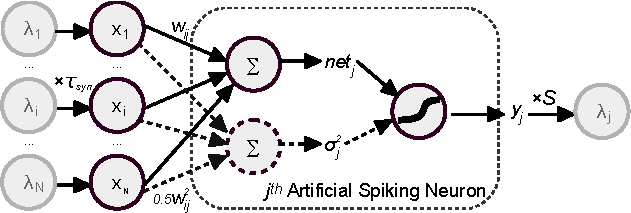
\includegraphics[width=0.8\textwidth]{pics_iconip/neuron_o.pdf}
	%	\caption{Artificial spiking neuron takes scaled firing rates as input, then transforms weighted sum in some activation unit to its output which can be scaled-up to the firing rate of an output spike train.}
	%	\label{Fig:sneuron}
	%\end{figure}
	%
	%Noisy Softplus transforms the noisy current with parameters of $(net_j, \sigma_j)$ to the equivalent ANN output $y_j$ , where it can be scaled up by the factor $S$ to the firing rate of SNNs.
	%Note that the calculation of noise level is not necessary for activation functions other than Noisy Softplus, for example, it can be set to a constant for Softplus or 0 for ReLU.
	%We name the neuron model `artificial spiking neurons' which takes firing rates of spike trains as input and output. 
	%The entire artificial spiking neuron model is then generalised to any ReLU/Softplus-like activation functions, See Figure~\ref{Fig:sneuron}.
	%
	%
	%
	%%	Figure~\ref{Fig:sneuron} shows an complete transformation process of a spiking neuron, which mimics the biological neurons taking and generating spike trains.
	%Referred to Figure~\ref{Fig:sneuron}, if we move the left end process of $\times \tau_{syn}$ to the right end after $\lambda_j$, Figure~\ref{Fig:sneuron} forms the same neuron model and structure as multilayer perceptron: neurons take $x$ as input and outputs $y$, and this conversion is illustrated in Figure~\ref{Fig:tneuron}.
	%The process within such an artificial neuron is divided into weighted summation and activation, which also applies to SNN modelling by combining the scaling factor $S$ and the synaptic time constant $\tau_{syn}$ to activation functions.
	%Thus the combined activation function for modelling SNNs should be:
	%\begin{equation}
	%y = f(x) \times S \times \tau_{syn}~~,
	%\label{equ:full_act}
	%\end{equation}
	%and its derivative function which is used when back propagates is:
	%\begin{equation}
	%\frac{\partial y}{\partial x} = f'(x) \times S \times \tau_{syn}~~.
	%\end{equation}
	%
	%\begin{figure}[tbh!]
	%	\centering
	%	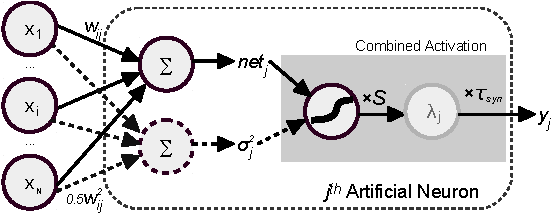
\includegraphics[width=0.8\textwidth]{pics_iconip/neuron_t.pdf}
	%	\caption{Transforming artificial spiking neurons to artificial neurons for SNN modelling. The combined activation links the firing activity of a spiking neuron to the numerical value of ANNs.}
	%	\label{Fig:tneuron}
	%\end{figure}
	
	\subsection{Generalised SNN Training}
	\label{subsec:ns_train}
	The simple change on activation functions presented in the previous section allows the use of common ANN training methods to obtain SNN-compatible weights.
	Consequently, training SNNs can be done in three simple steps: 
	\begin{enumerate}
		\item Calibrate the parameters $(k, S)$ for Noisy Softplus which models response firing rates of LIF neurons. Since $(k, S)$ are solely dependent on the biological configurations of an LIF neuron, the same parameters can be used for different activation functions and network architectures.
		\item Train any feed-forward ANN with a PAF version of an activation function. Training compatibility allows us to choose computationally simple activation functions to increase training speed. Surprisingly, the use of PAF-ReLU provides the best accuracy scores for an SNN on the MNIST dataset. 
		\item Transfer the weights directly to the SNN, which should use the same LIF characteristics used in Step 1.
	\end{enumerate}

	%Thus, once the parameters are tuned for a certain LIF configuration, they can be used for trainings with various activation functions.
	
	%todo
%	This generalised SNN training allows the use of widely-used activation functions in ANNs which are of low complexity and their corresponding derivative functions can be directly used for back propagation.
%	Especially, ReLU, the simplest and most effective activation function may improve the training performance of SNNs.
%	Ideally, the method can be applied for any feedforward network using ReLU-like activation functions, including deep architectures.
%	Most significantly, the ANN-trained weights are ready for use to transfer to SNNs without any conversion, and the output firing rate of a spiking neuron can be obtained in the ANN simulation thus to estimate the power use in Neuromorphic systems (hardware SNN simulators).
	
	
	
	\subsection{Fine Tuning}
	We can train the network with any PAF as stated above, and then fine-tune it with PAF-Noisy-Softplus to take account of both the accuracy and practical network activities of SNNs.
	The labels of data are always converted to binary values for ANN training.
	This enlarges the disparities between the correct recognition label and the rest to train the network for better classification capability.
	However, we add a small number, for example 0.01, to all the binary values of the data labels.
	Doing so helps the training to relax the strict objective function to predict exact labels with binary values.
	Instead, it allows a small offset to the objective.
	An alternative method is to use Softmax function at the top layer, which aims to map real vectors to the range $(0,1)$ that add up to 1. 
	However, without a limit on the input of Softmax, it will be easy to reach or even exceed the highest firing rate of a spiking neuron.
	The result of fine tuning on a Convnet will be demonstrated in subsection~\ref{subsec:result_compare}.
	
	There are two aspects to the fine tuning which make the ANN closer to SNNs:
	Firstly, using the Noisy Softplus activation functions causes every single neuron to run as a similar noise level as in SNNs, thus the weights trained by other activation functions will be tuned to fit closer to SNNs.
	Secondly, the output firing rate of any LIF neuron is greater than zero as long as noise exists in their synaptic input.
	Thus adding up a small offset on the labels directs the model to approximate practical SNNs. 
	
	\section{Results}
	\label{sec:result}
	
	\subsection{Experiment Set-up}
	A convolutional network model was trained on MNIST,
	%	~\cite{lecun1998gradient}
	a popular database in neuromorphic vision, using the generalised SNN training method stated above.
	The architecture contains $28\times28$ input units, followed by two convolution-pooling layers and 10 output neurons fully connected to the last pooling layer to represent the classified digit.
	
%	The training only employed Noisy Softplus units, which means all the convolution, average sampling, and the fully-connected neurons use Noisy Softplus function.
	The training employed PAFs and was compared with three core activation functions: ReLU, Softplus and Noisy Softplus.
	The parameter p was estimated as $p = S \times \tau_{syn} = 1.005$ by calibrating the Noisy Softplus with LIF response firing rate: $(k=0.30, S=201)$ given $\tau_{syn}=5 ms$.
	The pixel intensities of the input images were normalised to 100~\textit{Hz} to present the firing rates of the input spikes.
	The weights were updated using a decaying learning rate, 50 images per batch and 20 epochs.
	The ANN-trained weights were then directly transferred to the corresponding spiking ConvNet without any conversion for recognition tasks.
	
	
	\subsection{Neural Activity}
	To validate how well the Noisy Softplus activation fits to the response firing rate of LIF neurons in SNNs, we simulated the trained spiking ConvNet on NEST~\cite{gewaltig2007nest} using the Poisson MNIST dataset~\cite{liu2016bench}.
	
	A small test consisted of ten MNIST digits presented as Poisson spike trains for 1~s each.
	A PAF-Noisy-Softplus trained $5\times5$ kernel was convolved with these input digits, and the output firing rates were recorded and compared to the scaled activation functions: $S \times f(x)$.
	
	%The input $x$ of the network was calculated as Equation~\ref{equ:mi_input}: $x_i=\lambda_i\tau_{syn}$, and so as the weighted sum of the synaptic current (see Equation~\ref{equ:mi_input}), $net_j$ and its variance (see Equation~\ref{equ:si_input}), $\sigma^2_j$.
	%With three combined activation functions as Equation~\ref{equ:full_act}:
	%\begin{equation}
	%\begin{aligned}
	%&\textrm{(1) Noisy Softplus:~~}  y_j=k \sigma_j \log [1 + \exp(\frac{net_j}{k \sigma_j})] \times S \times \tau_{syn}~~,  \\
	%&\textrm{(2) ReLU:~~ } y_j=max(0, net_j) \times S \times \tau_{syn}~~, \\
	%&\textrm{(3) Softplus:~~ } y_j=k \sigma \log [1 + \exp(\frac{net_j}{k \sigma})] \times S \times \tau_{syn}~~, ~~~\sigma=0.45,  
	%\end{aligned}
	%\end{equation}	
%	With three PAFs of ReLU, Softplus and Noisy Softplus, we compare the output to the recorded SNN simulations.
	%ReLU assumes a non-noise current, and Softplus takes a static noise level thus $\sigma_j$ is not used for either of them, meanwhile Noisy Softplus adapts to noise automatically with $\sigma_j$.
	The experiment took the sequence of 10 digits to the same kernel and the estimated spike counts using Noisy Softplus fitted the real recorded firing rate much more accurately than ReLU and Softplus, see Figure~\ref{fig:af_compare}.
	%	Figure~\ref{fig:af_stast} illustrated the statistics of error between the estimation and the recorded firing rate, $err = y_j - \lambda_j$ which formed normal distributions where Noisy Softplus hold the weakest mean (low in abstract) and lowest standard deviation.
	The Euclidean distance, $\sqrt{\sum_{j}(y_j/\tau_{syn} - \lambda_j)^2}$, between the spike counts and the predicted firing rates by Noisy Softplus, ReLU and Softplus was 184.57, 361.64 and 1102.76 respectively.
	We manually selected a static noise level of 0.45 for Softplus, whose estimated firing rates located roughly on the top slope of the real response activity.
	This resulted in a longer Euclidean distance than using ReLU, since most of the input noisy currents were of relatively low noise level in this experiment.
	Hence, the firing rate driven by the lower noise level is closer to ReLU curve than Softplus.
	
	\begin{figure}[hb!]
		\centering
		\begin{subfigure}[hb]{0.32\textwidth}
			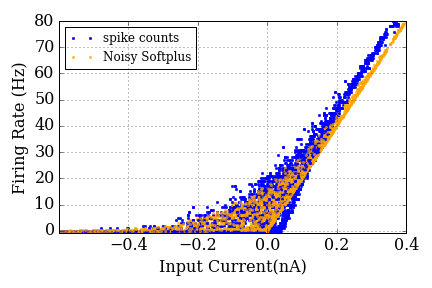
\includegraphics[width=\textwidth]{pics_iconip/6-5-3.png}
			\caption{Softplus}
		\end{subfigure}
		\begin{subfigure}[hb]{0.32\textwidth}
			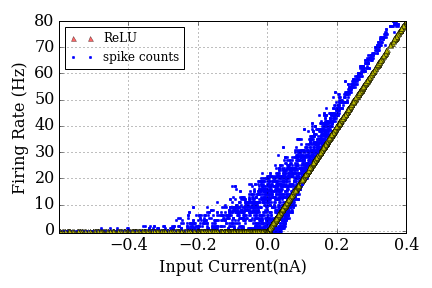
\includegraphics[width=\textwidth]{pics_iconip/6-5-2.png}
			\caption{ReLU}
		\end{subfigure}
		\begin{subfigure}[hb]{0.32\textwidth}
			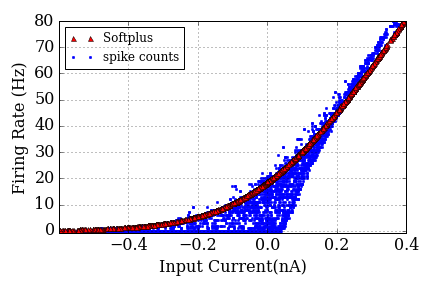
\includegraphics[width=\textwidth]{pics_iconip/6-5-1.png}
			\caption{Noisy Softplus}
		\end{subfigure}
		\caption{
			The recorded firing rate of the convolution of the same kernel with 10 images in SNN simulation, compared to the firing rate prediction by $S \times f(x)$.
			Noisy Softplus (a) fits to the neural response firing rate of LIF neurons more closely than ReLU (b) and Softplus (c).}
		\label{fig:af_compare}
	\end{figure}		
	
%	The SNN successfully classified the digits where the correct label neuron fired the most.
%	We trained the network with binary labels on the output layer, thus the expected firing rate of correct classification was $1/\tau_{syn}=200$~\textit{Hz} according to Equation~\ref{Fig:tneuron}.
%	The firing rates of the recognition test fell to the valid range around 0 to 200~\textit{Hz}.
	This shows another advantage of the Noisy Softplus activation function that we can estimate the firing rate of an SNN by $S \times f_{NS}(x)$ running its equivalent ANN, instead of simulating SNNs.
	Moreover, we can constrain the expected firing rate of the top layer, thus preventing the SNN from exceeding its maximum firing rate, for example 1000~\textit{Hz} when the time resolution of the SNN simulation is set to 1~ms.
	
	
	\subsection{Learning Performance}
	%Here we focus on the recognition performance of the proposed ANN-trained SNN method.
	Before looking into the recognition results, it is significant to see the learning capability of the proposed activation function, Noisy Softplus.
	We compared the training using ReLU, Softplus, and Noisy Softplus by their loss during training averaged over 3 trials, see Figure~\ref{Fig:loss_ns}.
	ReLU learned fastest with the lowest loss, thanks to its steepest derivative.
	In comparison, Softplus accumulated spontaneous firing rates layer by layer and its derivative may experience vanishing gradients during back propagation, which result in a more difficult training.
	The Noisy Softplus performance lay between these two in terms of loss and learning speed.
	However, the loss stabilised fastest, which means a possibly shorter training time.
	%\begin{figure}[tbp!]
	%	\centering
	%	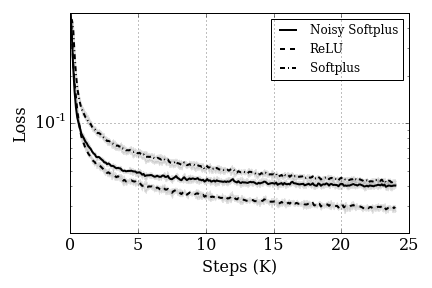
\includegraphics[width=0.7\textwidth]{pics_iconip/8.png}
	%	\caption{Comparisons of Loss during training using Noisy Softplus, ReLU and Softplus activation functions. Bold lines show the average of three training trials, and the grey colour illustrates the range between the minimum and the maximum values of the trials.  }
	%	\label{Fig:loss_ns}
	%\end{figure}
	%	The trained networks were scaled to SNNs and compared on recognition rates, 93.34\%, 96.43\% and 97.03\% with a conversion loss of 4.76\%, 0.91\% and 0.74\%.
	
	\begin{figure}
		\begin{minipage}[t]{0.48\linewidth}
			\raggedleft
			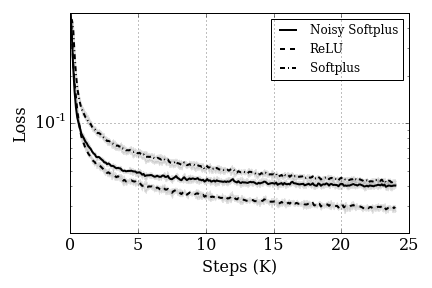
\includegraphics[width=2.6in]{pics_iconip/8.png}
			\caption{Comparisons of Loss during training using PAF version of Noisy Softplus, ReLU and Softplus. Bold lines show the average of three training trials, and the grey colour illustrates the range between the minimum and the maximum values of the trials. }
			\label{Fig:loss_ns}
		\end{minipage}%
		\hspace{0.04\linewidth}
		\begin{minipage}[t]{0.48\linewidth}
			\raggedright
			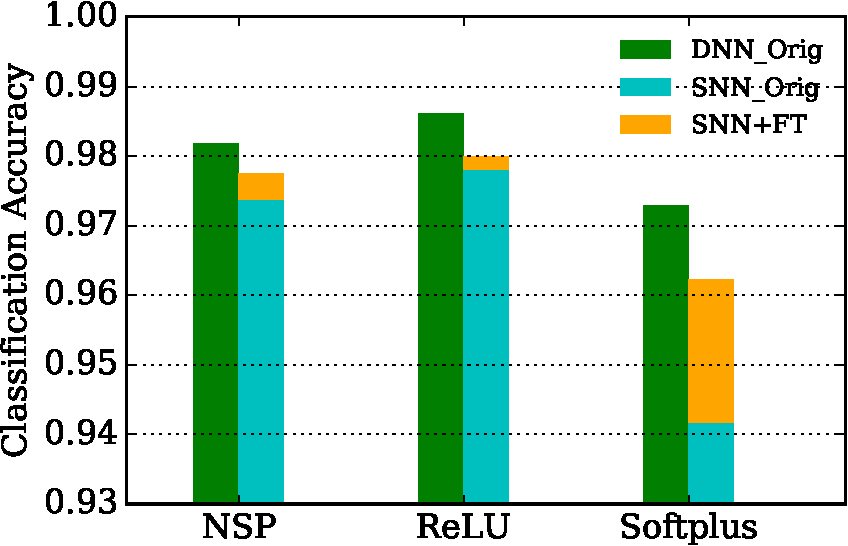
\includegraphics[width=2.6in]{pics_iconip/9-2.pdf}
			\caption{Classification accuracy.
			The trained weights were tested using the same activation function as training (DNN\_Orig), then tested using Noisy Softplus (DNN\_NS) and transferred to SNN test (SNN\_Orig), and finally fine-tuned to be tested using Noisy Softplus (DNN+FT\_NS) and on SNN simulation (SNN\_FT).  }
			\label{Fig:result_bar}
		\end{minipage}
	\end{figure}
	
	\subsection{Recognition Performance}
	\label{subsec:result_compare}
	The recognition test took the whole testing dataset of MNIST which contains $10,000$ images.
	At first, all trained models were tested on the same artificial neurons as used for training in ANNs, and these experiments were called the `DNN' test since the network had a deep structure (6 layers).
	Subsequently, the trained weights were directly applied to the SNN without any transformation, and these `SNN' experiments tested their recognition performance on the NEST simulator.
	The LIF neurons had the same parameters as in training.
	The input images were converted to Poisson spike trains and presented for 1~s each.
	The output neuron which fired the most indicated the classification of an input image.
	Moreover, a `fine tuning' test took the trained model for fine tuning, and the tuned weights were tested on the same SNN environment.
	The tuning only ran for one epoch, 5\% of the cost of the ANN training (20~epochs), using Noisy Softplus neurons with labels shifted by $+0.01$.
	
	The classification errors for the tests are investigated by comparing the average classification accuracy, shown in Figure~\ref{Fig:result_bar}.
	From DNN to SNN, the classification accuracy declines by 0.80\%, 0.79\% and 3.12\% on average for Noisy softplus, ReLU and Softplus
	The accuracy loss was caused by the mismatch between the activations and the practical response firing rates, see example in Figure~\ref{fig:af_compare}, and the strict binary labels for Noisy Softplus and Softplus activations.
	Fortunately, the problem is alleviated by fine tuning which increased the classification accuracy by 0.38\%, 0.19\% and 2.06\%, and resulted in the total loss of 0.43\%, 0.61\%, and 1.06\% respectively.
  
	As the recognition performance of ReLU is already high, there's little room for improvement. Even though the fine-tuning procedure does its job, the gain in accuracy is the smallest for this activation function.
	
  %	Thus fine tuning mainly corrects the mismatch between ReLU and the firing rates in SNNs, and constraints the output firing rates of the network.
	Softplus benefits the most from fine tuning, since not only the huge mismatch of response firing rate is greatly corrected, but also the offset on the labels helps the network to fit SNNs. 
	%dummy change
	%\begin{figure}[hbt!]
	%	\centering
	%	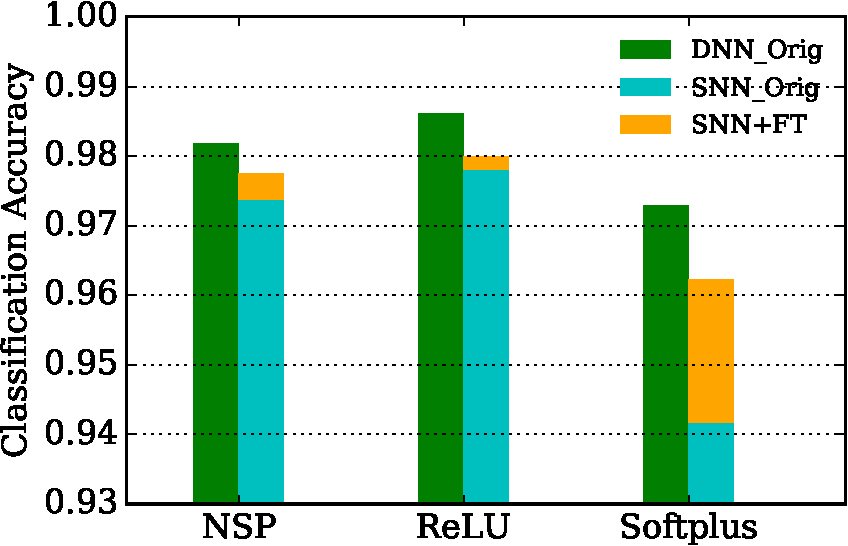
\includegraphics[width=0.7\textwidth]{pics_iconip/9-2.pdf}
	%	\caption{Classification accuracy compared among trained weights of Noisy Softplus, ReLU, Softplus on DNN, SNN and fine-tuned SNN.}
	%	\label{Fig:result_bar1}
	%\end{figure}
	
	%\begin{table}[tbh] 
	%	\caption{Comparisons of classification accuracy (in \%) of ANN-trained convolutional neural models on original DNN, NEST simulated SNN, and SNN with fine-tuned (FT) model.}
	%	\begin{center}
	%		\bgroup
	%		\def\arraystretch{1.5}
	%		\begin{tabular} {r |c  c c |c c c |c c c}
	%			%First line
	%			\hline
	%			Trial No.
	%			&\multicolumn{3}{c|}{1} 
	%			&\multicolumn{3}{c|}{2}
	%			&\multicolumn{3}{c}{3}\\
	%			\hline
	%			Model
	%			& DNN & SNN &FT
	%			& DNN & SNN &FT
	%			& DNN & SNN &FT\\
	%			\hline
	%			\textbf{Noisy Sofplus}
	%			& 1.91 & 2.76 &2.45
	%			& 1.79 & 2.56 &2.19
	%			& 1.76 & 2.55 &2.10\\
	%			%				& 98.09 & 97.24 &97.55
	%			%				& 98.21 & 97.44 &97.81
	%			%				& 98.24 & 97.45 &97.90\\
	%			%				\hline
	%			\textbf{ReLU}
	%			& 1.36 & 2.03 &1.88
	%			& 1.46 & 2.28 &2.00
	%			& 1.36 & 2.25 &2.12\\
	%			%				& 98.64 & 97.97 &98.12
	%			%				& 98.54 & 97.72 &98.00
	%			%				& 98.64 & 97.75 &97.88\\
	%			%				\hline
	%			\textbf{Sofplus}
	%			& 2.30 & 5.66 &3.91
	%			& 2.75 & 5.22 &3.55
	%			& 2.42 & 6.62 &3.87\\
	%			%				& 97.70 & 94.34 &96.09
	%			%				& 97.25 & 94.78 &96.45
	%			%				& 97.58 & 93.38 &96.13\\
	%			\hline
	%		\end{tabular}
	%		\egroup
	%		\label{tbl:ns_result}
	%	\end{center}
	%\end{table}
	
	
	
	
	%	The best classification accuracy achieved by SNNs was trained with ReLU and fine-tuned by Noisy Softplus.
	The most efficient training in terms of both classification accuracy and algorithm complexity, takes ReLU for ANN training and Noisy Softplus for fine tuning.
	Softplus does not exhibit better classification capability and, more importantly, the manually selected static noise level hugely influences the mismatch between the predicted firing rates and the real data.
	Although Noisy Softplus shows the least classification drop from ANNs to SNNs, the training performance is still worse than ReLU.
	%	Improved back propagation or other learning algorithms using noise level will be listed in the future work. 
	
	The best classification accuracy achieved by an SNN was 98.85\%, a 0.20\% drop from the ANN test (99.05\%), which was trained with ReLU and fine-tuned using Noisy Softplus.
	It is useful to compare with existing SNN training methods in Table~\ref{tbl:compare} where we order them on the computation complexity (descending).
	The generalised training method this paper proposed wins over the simplest activation function, and no conversions are requited of trained weights to be transferred to SNNs, they are well fitted to biologically-plausible LIF neurons, and only an optional additive processing of fine tuning.
	
	
	
  \begin{table*}[thb!]
	\caption{SNN training methods comparison.}
	\begin{center}
		\bgroup
		\def\arraystretch{1.1}
		\begin{tabular}{l c c c c c c}
			\begin{mycell}{1cm} Method \end{mycell} & 
			%  					\begin{mycell}{1.8cm} Computation\\Complexity \end{mycell} & 
			\begin{mycell}{1.8cm}Activation\\Function\end{mycell} &
			\begin{mycell}{1.8cm} Biologically-\\plausibility \end{mycell} &  
			\begin{mycell}{1.8cm} Additional\\Processing \end{mycell} &
			\begin{mycell}{1.8cm} Conversion \end{mycell} & 
			\begin{mycell}{1.8cm} Classification\\Accuracy(\%) \end{mycell} 
			\\
			\hline
			\begin{mycell}{1cm} \cite{Jug_etal_2012} \end{mycell} & 
			%  					\begin{mycell}{1.8cm} 1st \end{mycell} & 
			\begin{mycell}{1.8cm}Siegert \end{mycell} &
			\begin{mycell}{1.8cm} \textbf{Yes} \end{mycell} &  
			\begin{mycell}{1.8cm} \textbf{No} \end{mycell} & 
			\begin{mycell}{1.8cm} \textbf{No} \end{mycell} & 
			\begin{mycell}{1.8cm} 94.94~\cite{Stromatias2015scalable} \end{mycell} 
			\\
			\begin{mycell}{1cm} \cite{hunsberger2015spiking} \end{mycell} & 
			%  					\begin{mycell}{1.8cm} 2nd \end{mycell} & 
			\begin{mycell}{1.8cm} Soft LIF \end{mycell} &
			\begin{mycell}{1.8cm} \textbf{Yes} \end{mycell} &  
			\begin{mycell}{2.2cm} Noisy inputs\\ \&Activations \end{mycell} & 
			\begin{mycell}{1.8cm} \textbf{No} \end{mycell} & 
			\begin{mycell}{1.8cm} 98.37 \end{mycell}
			\\
			\begin{mycell}{1cm} \cite{diehl2015fast} \end{mycell} & 
			%  					\begin{mycell}{1.8cm} 3rd \end{mycell} & 
			\begin{mycell}{1.8cm} \textbf{ReLU} \end{mycell} &
			\begin{mycell}{1.8cm} No \end{mycell} &  
			\begin{mycell}{1.8cm} Dropout  \end{mycell} & %\&\\Conversion
			\begin{mycell}{1.8cm} Yes \end{mycell} &  
			\begin{mycell}{1.8cm} \textbf{99.1\%} \end{mycell} 
			\\
			\begin{mycell}{1cm} This\\Paper \end{mycell} & 
			%  					\begin{mycell}{1.8cm} 3rd \end{mycell} & 
			\begin{mycell}{1.8cm} \textbf{PAF}\\($p\times$ReLU)\end{mycell} &
			\begin{mycell}{1.8cm} \textbf{Yes} \end{mycell} &  
			\begin{mycell}{2.2cm} \textbf{No} \\or fine tune  \end{mycell} & 
			\begin{mycell}{1.8cm} \textbf{No} \end{mycell} & 
			\begin{mycell}{2.4cm} 98.70\\ 98.85(fine tune) \end{mycell}  
			% contents!
		\end{tabular}
		\egroup
	\end{center}
	\label{tbl:compare}
\end{table*}
	
	%The network structure was the same with the state-of-the-art model which reported the best classification accuracy of 99.1\%~\cite{diehl2015fast} in ANN-trained SNNs: 12c5-2s-64c5-2s-10fc.
	%Their nearly loss-less conversion from ANNs to SNNs was achieved by using IF neurons, while our network performs the best among SNNs consisted of LIF neurons to our knowledge.
	
	\begin{figure}[htb!]
		\centering
		\begin{subfigure}[t]{0.49\textwidth}
			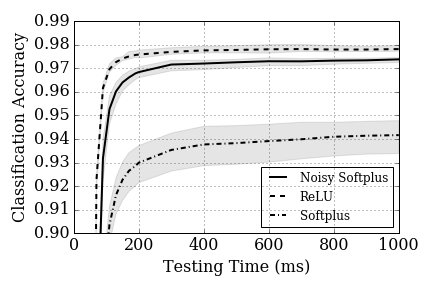
\includegraphics[width=\textwidth]{pics_iconip/8-2.png}
			\caption{Before fine tuning}
		\end{subfigure}
		\begin{subfigure}[t]{0.49\textwidth}
			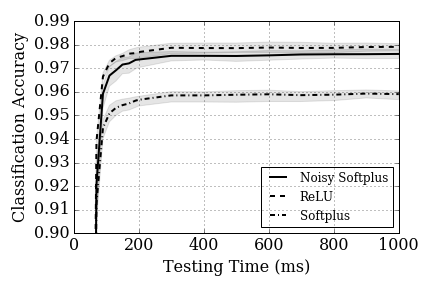
\includegraphics[width=\textwidth]{pics_iconip/8-3.png}
			\caption{After fine tuning.}
		\end{subfigure}
		
		\caption{The classification accuracy of 3 trials (averaged in bold lines, grey shading shows the range between minimum to maximum) over short response times, with (a) trained weights before fine tuning, and (b) after fine tuning.}
		\label{fig:ca_time}	
	\end{figure}
	
	As it is a major concern in neuromorphic vision, the recognition performance over short response times is also estimated in Figure~\ref{fig:ca_time}.
	After fine tuning, Softplus significantly reduced the mismatch since the randomness among the three trials shrinks to a range similar to other experiments.
	Fine tuning also improved its classification accuracy and the response latency.
	Notice that all of the networks trained by three different activation functions showed a very similar stabilisation curve against time, which means they all reached an accuracy close to their best after only 300~ms. 
	
	
	\subsection{Power Consumption}
	Neuromorphic engineering aims to build intelligent machines with low power cost, thus power consumption is an important metric for evaluating their performance~\cite{liu2016bench}.
	PAF provides energy estimation for SNNs without running the models on real neuromorphic hardware.
	For a single neuron, the energy consumption of the synaptic events it triggers is:
	\begin{equation}
	E_{j} = \lambda_j N_j T E_{syn} = \dfrac{y_j N_j T E_{syn}}{\tau_{syn}}~~,
	\label{equ:energy}
	\end{equation}
	where $\lambda_j$ is the output firing rate, $N_j$ is the number of post-synaptic neurons it connects to, $T$ is the testing time, and $E_{syn}$ is the energy cost for a synaptic event of some specific neuromorphic hardware, for example, about 8~nJ on SpiNNaker~\cite{stromatias2013power}.
	Thus to estimate the whole network, we can sum up all the synaptic events of all the neurons:
	\begin{equation}
	\sum_j E_{j} =  \dfrac{T E_{syn}}{\tau_{syn}} \sum_{j}y_j N_j.
	\end{equation}
	Thus, it may cost SpiNNaker 0.064~W, 192~J running for $3,000$~s with synaptic events of $8\times10^6/s$ to classify $10,000$ images (300~ms each) with an accuracy of 98.02\%.
	The best performance reported using the larger network may cost SpiNNaker 0.43~W operating synaptic event rate at $5.34\times10^7/s$, consuming 4271.6~J to classify all the images for 1~s each.
	
	\section{Conclusion and Future Work}
	We presented a generalised SNN training method to train an equivalent ANN and transfer the trained weights back to SNNs.
	This training procedure consists of two simple stages: first, estimate parameter $p$ for PAF using Noisy Softplus, and second, use a PAF version of conventional activation functions for ANN training. % can be generalised to activation units other than Noisy Softplus.
	%The training of a SNN model is exactly the same as ANN training, and 
	The trained weights can be directly used in SNN without any further transformation.
	This method requires the least computation complexity while performing most effectively among existing training algorithms.
	% and even more straight-forward than the other ANN offline training methods which requires an extra step of converting ANN-trained weights to SNN's.
	
	In terms of classification/recognition accuracy, the performance of ANN-trained SNNs is nearly equivalent to ANNs, and the performance loss can be partially solved by fine tuning.
	The best classification accuracy of 98.85\% using LIF neurons in a PyNN simulation outperforms state-of-the-art SNN models of LIF neurons and is very close to the result using IF neurons~\cite{diehl2015fast}.
	
	The current limitation prohibiting this off-line SNN training method from wide use lies in the lack of supporting tools, which would enable SNN training on popular deep learning platforms. Additionally an automation tool to read platform-dependent trained weights into the PyNN~\cite{davison2008pynn} language.
	Another issue is the parameter calibration on the scaling factor of the PAF, thus numerical analysis is considered for future work to express the factors with biological parameters of a LIF neuron.
	Interesting applications have started with collaborations on speech recognition of cochlea generated spikes which has achieved a promising accuracy at the initial test-idea stage.
%	A further goal is to implement deep networks fit for ImageNet~\cite{deng2009imagenet} tasks, which will also require modelling various structures of deep learning, for example recurrent neural networks.
	
	\section*{Acknowledgments}
	To be added after reviewing.
	%The work presented in this paper was largely inspired by discussions at the 2015 Workshops on Neuromorphic Cognition Engineering in CapoCaccia.The authors would like to thank the organisers and the sponsors.The authors would also like to thank Patrick Camilleri, Michael Hopkins, and Viv Woods for meaningful discussions and proof-reading the paper.The construction of the SpiNNaker machine was supported by the Engineering and Physical Sciences Research Council (EPSRC grant EP/4015740/1) with additional support from industry partners ARM Ltd and Silistix Ltd.The research leading to these results has received funding from the European Research Council under the European Union's Seventh Framework Programme (FP/2007-2013) / ERC Grant Agreement n. 320689 and from the EU Flagship Human Brain Project (FP7-604102). The research leading to these results has received funding from Natural Science Foundation of Guangdong Province, China (No: 2016A030313713) and also from  Natural Science Foundation of Guangdong Province, China (No: 2014A030310169).
	
	%The research leading to these results has received funding from the European Research Council 
	%(FP/2007-2013) / ERC Grant Agreement n. 320689 and from the EU Flagship Human Brain Project (FP7-604102). 
	%Yunhua Chen received funding from the Natural Science Foundation of Guangdong Province, China (No: 2016A030313713) and also from  the Natural Science Foundation of Guangdong Province, China (No: 2014A030310169).
	%Qian Liu personally thanks to the funding from the National Natural Science Foundation of China (61662013,U1501252), the Guangxi Natural Science Foundation~(2014GXNSFDA118036), and The High Level of Innovation Team of Colleges and Universities in Guangxi and Outstanding Scholars Program Funding.
	
	\small
	
	\bibliographystyle{unsrt}
	\bibliography{ref}
\end{document}